\chapter{\ccclr{}: Additional Materials}\label{chap:c3lr-additional-mat}

This chapter deals with the justification of certain design choices made for \ccclr{} (\Cref{chap:c3lr-art}), that could not be covered in the original article due to space constraints.
The algorithm in the article is made available here for convenience.
\begin{algorithm}[ht]
    \caption{\scalebox{.9}{Class-Cognizant Contrastive Learning (\ccclr{})}}\label{alg:pclr-c}
    
    % \setstretch{.8}
    \SetAlgoSkip{}
    \SetKwInOut{Input}{input}
    \SetKwInOut{Output}{output}
    \SetKwInput{Require}{Require}
	\SetKwInput{Return}{Return}
	\SetKw{Let}{let}
	\SetKwRepeat{Do}{do}{while}
	
	\SetAlgoLined
	\LinesNumbered
	\DontPrintSemicolon
	\SetNoFillComment
    \Require{$L$, $Q$, $f_\phi$, $\mathcal{A}$, $\alpha$, $d[\cdot, \cdot]$}

    \While {not done}{
        Sample minibatch $\left\{\symbfit{x}_{i}\right\}_{i=1}^{L}$\;
        \ForAll{$i \in\{1, \ldots, L\}$} {
            \ForAll{$q \in\{1, \ldots, Q\}$}{
                $\tilde{\symbfit{x}}_{i, q}=\psi^{q}(\symbfit{x}_{i})$; $\psi^{q} \sim \mathcal{A}$.\;  
            }
        }
        $\symbf{R} = \texttt{ReRank}$\scalebox{.8}{$\left(\left[ f_{\phi }\left(\{\symbfit{x}_{i}\}_{i=1}^{L}\right) ,f_{\phi }\left(\left\{\tilde{\symbfit{x}}_{i,\ q}\right\}_{i=1,q=1}^{L,Q}\right)\right]\right)$}\; 
        
        
        $\mathcal{C} = \{\symbfit{C}_1 ,\symbfit{C}_2 ,\dotsc ,\symbfit{C}_{P}\} \gets \texttt{HDBSCAN}(\symbf{R})$\;
        
        
        $\mathcal{M} = \{{\symbf m}_{p}\}_{p = 1}^P;$ \hspace{0.1cm} ${\symbf m}_p = \frac{\sum _{x_{j} \in \symbfit{C}_{p}} x_{j}}{|\symbfit{C}_{p} |}$\;
        
        \vspace{0.15cm}
        \Let{\scalebox{.95}{$\mathscr{r} (i,q,p)=-\log\frac{\exp\left( -d\left[ f_\phi\left(\tilde{{\symbfit x}}_{i,q}\right) ,\symbf{m}_{p}\right]\right) }{\sum_{p=1}^{P}\exp\left( -d\left[ f_\phi\left(\tilde{\symbfit{x}}_{i,q}\right) ,\symbf{m}_{p}\right]\right)}$}}\;
        \vspace{+0.15cm}
        \Let{\scalebox{.95}{$\ell(i, q)=-\log \frac{\exp \left(-d\left[f_\phi\left(\tilde{{\symbfit x}}_{i, q}\right), f_\phi\left(\symbfit{x}_{i}\right)\right]\right)}{\sum_{k=1}^{L} \exp \left(-d\left[f_\phi\left(\tilde{{\symbfit x}}_{i, q}\right), f_\phi\left(\symbfit{x}_{k}\right)\right]\right)}$}}\;
        
        \vspace{+0.15cm}
        $\mathcal{L}_{1}=\frac{1}{L Q} \sum_{p=1}^{P} \sum_{i=1}^{L} \sum_{q=1}^{Q} \mathscr{r}(i, q, p)$\;
        $\mathcal{L}_{2}=\frac{1}{L Q} \sum_{i=1}^{L} \sum_{q=1}^{Q} \ell(i, q)$\;
        
        $\mathcal{L} = \mathcal{L}_{1} + \mathcal{L}_{2}$
        
        $\phi \gets \phi-\alpha \nabla_{\phi} \mathcal{L}$\;
    }
\end{algorithm}


\section{Choice of Clustering Algorithm}\label{sec:c3lr-clustering-algo}

As we can see from \Cref{alg:pclr-c} and \cref{chap:c3lr-art}, the re-ranking and clustering steps are crucial to its functioning. The purpose of this section is to show why \texttt{HDBSCAN} \parencite{McInnes2017Hdbscan:Clustering} was chosen in combination with the $k$-reciprocal Jaccardian distance \parencite{ZhongRe-rankingEncoding}. To motivate our choices, we shall refer to \cref{tab:c3lr-combos}.

\begin{table}[!ht]
    \centering
    {\tabcolsep=0pt\def\arraystretch{1.1}
    \begin{tabularx}{\textwidth}{l >{\centering\arraybackslash}p{90pt} *4{@{}Y} >{\centering\arraybackslash}p{80pt}}
    \toprule
        \textbf{Method} & Clustering Algorithm  & UMAP & UMAP $\mathbb{R}^{\symbf \cdot}$ & $L$ & $B$ & Avg Test Acc ($\%$)\\ 
        \midrule
        ProtoCLR & None & \xmark & -  & 50 & 200 & 60.66 \\
        ProtoCLR & None & \xmark & - & 200 & 800 & 62.32 \\
        % \ccclr{}         & None & Pairwise & \xmark & - & 50 & 200 & 58.42 \\ 
        % \ccclr{}         & None & Pairwise & \xmark & - & 50 & 200 & 46.06 \\
        % \ccclr{}         & None & Pairwise & \xmark & - & 50 & 400 & 57.22 \\
        % \ccclr{}         & None & Centroid & No & - & 10 & 5 & 50 & 200 & 54.05 \\ 
        % \ccclr{}         & None & Centroid & No & - & 10 & 10 & 100 & 400 & 63.24 \\
        % \ccclr{}         & None & Centroid & No & - & 20 & 5 & 100 & 400 & 58.36 \\ 
        % \ccclr{}         & None & Centroid & No & - & 5 & 20 & 100 & 400 & 60.73 \\ 
        % \ccclr{}         & None & Centroid & No & - & 10 & 20 & 200 & 800 & 65.34 \\ 
        \ccclr{} (Oracle)        & None & \xmark & - & 200 & 800 & \textbf{66.86} \\ 
        \ccclr{}         & $K$-means ($K=5$)    & \cmark & 3 & 200 & 800 & 62.14 \\ 
        \ccclr{}         & $K$-means ($K=5$)    & \xmark & -  & 200 & 800 & 62.19 \\
        \ccclr{}         & $K$-means ($K=10$)   & \xmark & -  & 200 & 800 & 61.69 \\
        \ccclr{}         & $K$-means ($K=25$)   & \cmark & 3 & 200 & 800 & 62.68 \\
        \ccclr{}         & $K$-means ($K=25$)   & \xmark & -  & 200 & 800 & 63.60 \\ 
        \ccclr{}         & HDBSCAN          & \cmark & 3  & 200 & 800 & 62.46 \\
        \ccclr{}         & HDBSCAN          & \xmark & -  & 200 & 800 & 62.44 \\
        \ccclr{}         & HDBSCAN + $k$-rJd & \cmark & 2  & 200 & 800 & 63.79 \\
        \ccclr{}         & HDBSCAN + $k$-rJd & \xmark & - & 200 & 800 & \underline{64.81} \\
        \bottomrule
    \end{tabularx}}
    \caption{Table comparing design choices for \ccclr{} though accuracy ($\%$) on (\nwks{5}{5}) classification tasks. $L$ is number of source images, $B$ is the total number of images including augmentations. Style: \textbf{best} and \underline{second best}.}
    \label{tab:c3lr-combos}
\end{table}

\cref{tab:c3lr-combos} shows the performance of \ccclr{} with $K$-means and \texttt{HDBSCAN} as clustering algorithms of choice. The best performing variant of \ccclr{} is the \textbf{oracle} variant, this variant of the model provided access to the true labels of the data. The true labels allowed the creation of the ideal cluster centres. To understand why this is, we shall elaborate on lines $9$ and $10$ in \cref{alg:pclr-c}. In line $9$, \texttt{HDBSCAN} processes the embeddings and groups them, when we say that an element belongs to cluster $\symbf{C}_p$ it also implies that $\symbf{C}_p$ functions as a predicted label for that element. 
Instead of using predicted labels, the oracle variant uses actual labels. Since we know the actual grouping of elements, we can calculate the ideal cluster centres on line $10$. 
The purpose of the oracle model is to gauge the potential maximum performance that could be achieved using the training algorithm in question if the model were given all available label information without changing any other aspects of the training algorithm. 
It gives us a theoretical maximum that we know the training regime is capable of reaching. Ideally we want non-oracle models to be as close as possible to the performance of the oracle variant.

As shown in \cref{tab:c3lr-combos}, the $K$-means algorithm has been tested with various values of $K$. We tried values of $K$ that seemed reasonable; however, the results were not promising and were the same as that of ProtoCLR. The choice of $K$ was kept to at most $25$, because we wanted a cluster to have sufficient samples for the calculation of loss $\mathcal{L}_1$.
Choosing the ideal value for $K$ is also an additional overhead; for example, a value of $K$ that works well with \miniImagenet{} may not work well for \tieredImagenet{}.
We were unable to test the combination of $K$-means with $k$-reciprocal Jaccardian distance ($k$-rJd) because the implementation of $K$-means in Scikit-learn does not take a custom distance matrix as input \parencite{scikit-learn}.

With the shortcomings of $K$-means in mind, we wanted to use a smarter clustering algorithm that could take custom distance matrices and automatically discover the ideal number of clusters in a given batch of size $B$. We decided to explore \texttt{HDBSCAN} \parencite{McInnes2017Hdbscan:Clustering} as it can find clusters with variable densities and is also less prone to noise than DBSCAN \parencite{ester1996density,schubert2017dbscan}. 

Choosing \texttt{HDBSCAN} did not immediately pay off; however, we did notice that the performance of \ccclr{} was more stable with \texttt{HDBSCAN} since we no longer needed to determine the optimal number of clusters required by trial and error. 
The stability given to us by \texttt{HDBSCAN} gave us the confidence to investigate other changes in \ccclr{} that could improve performance. A natural thought was to refine the neighbourhood of each sample so that it is close to elements that are similar to itself, since this would allow \texttt{HDBSCAN} to discover better clusters. Therefore, we took inspiration from the method developed by \textcite{Ji2019UnsupervisedTraining} and utilised $k$-reciprocal Jaccardian distance ($k$-rJd) based re-ranking of elements \parencite{ZhongRe-rankingEncoding}. $k$-rJd takes into account the reciprocal relationship between data points and is therefore a stricter rule to measure whether two feature vectors match or not, thereby aiding \texttt{HDBSCAN} in finding better clusters.

It is well known that both $K$-means and \texttt{HDBSCAN} suffer from the curse of dimensionality \parencite{Kriegel09, McInnes2017Hdbscan:Clustering}; to mitigate the effects of dimensionality, we explored the use of UMAP \parencite{mcinnes2018umap} prior to the re-ranking and clustering steps on the lines $8-9$.
The idea was to apply UMAP to $f_\phi(\symbfit{x}) \in \mathbb{R}^{1600}$ and reduce the dimensionality to $\mathbb{R}^3$ or $\mathbb{R}^2$.
Unfortunately, we did not see significant performance improvements. The results of this are also given in \cref{tab:c3lr-combos}. The column \textquote{UMAP $\mathbb{R}^{\symbf \cdot}$} refers to the number of UMAP dimensions.

\section{Shortcomings of \ccclr{}}\label{sec:c3lr-shortcomes}

Although \ccclr{} is better than its competitors, it still has some shortcomings that we shall discuss in this section.

\subsection{Unstable Clusters}\label{ssec:unstable-clusters}

As discussed in \cref{sec:c3lr-clustering-algo}, we decided to use \texttt{HDBSCAN} as it provided a \textit{relatively} more stable performance than $K$-means. However, \texttt{HDBSCAN} frequently generated massive clusters, as there is no way to constrain how many elements can be placed in a cluster. This meant that members of certain clusters were not really similar, leading to a sub-optimal effect of loss $\mathcal{L}_1$ on the learning process. From \cref{fig:c3lr-hdbscan-results,fig:hdbscan-noise-count} we can see that the sheer number of points classified as noise hovers around the $400$ mark. It must be noted that \ccclr{} has an effective batch size $B=800$, which means that in every training iteration roughly half of the data was discarded as noise by \texttt{HDBSCAN}. Only the remaining amount of data played an active role in the calculation of $\mathcal{L}_1$.
Moreover, running the \texttt{HDBSCAN} algorithm for every batch is a time-consuming and computationally heavy process.
\begin{figure}[ht]
    \centering
    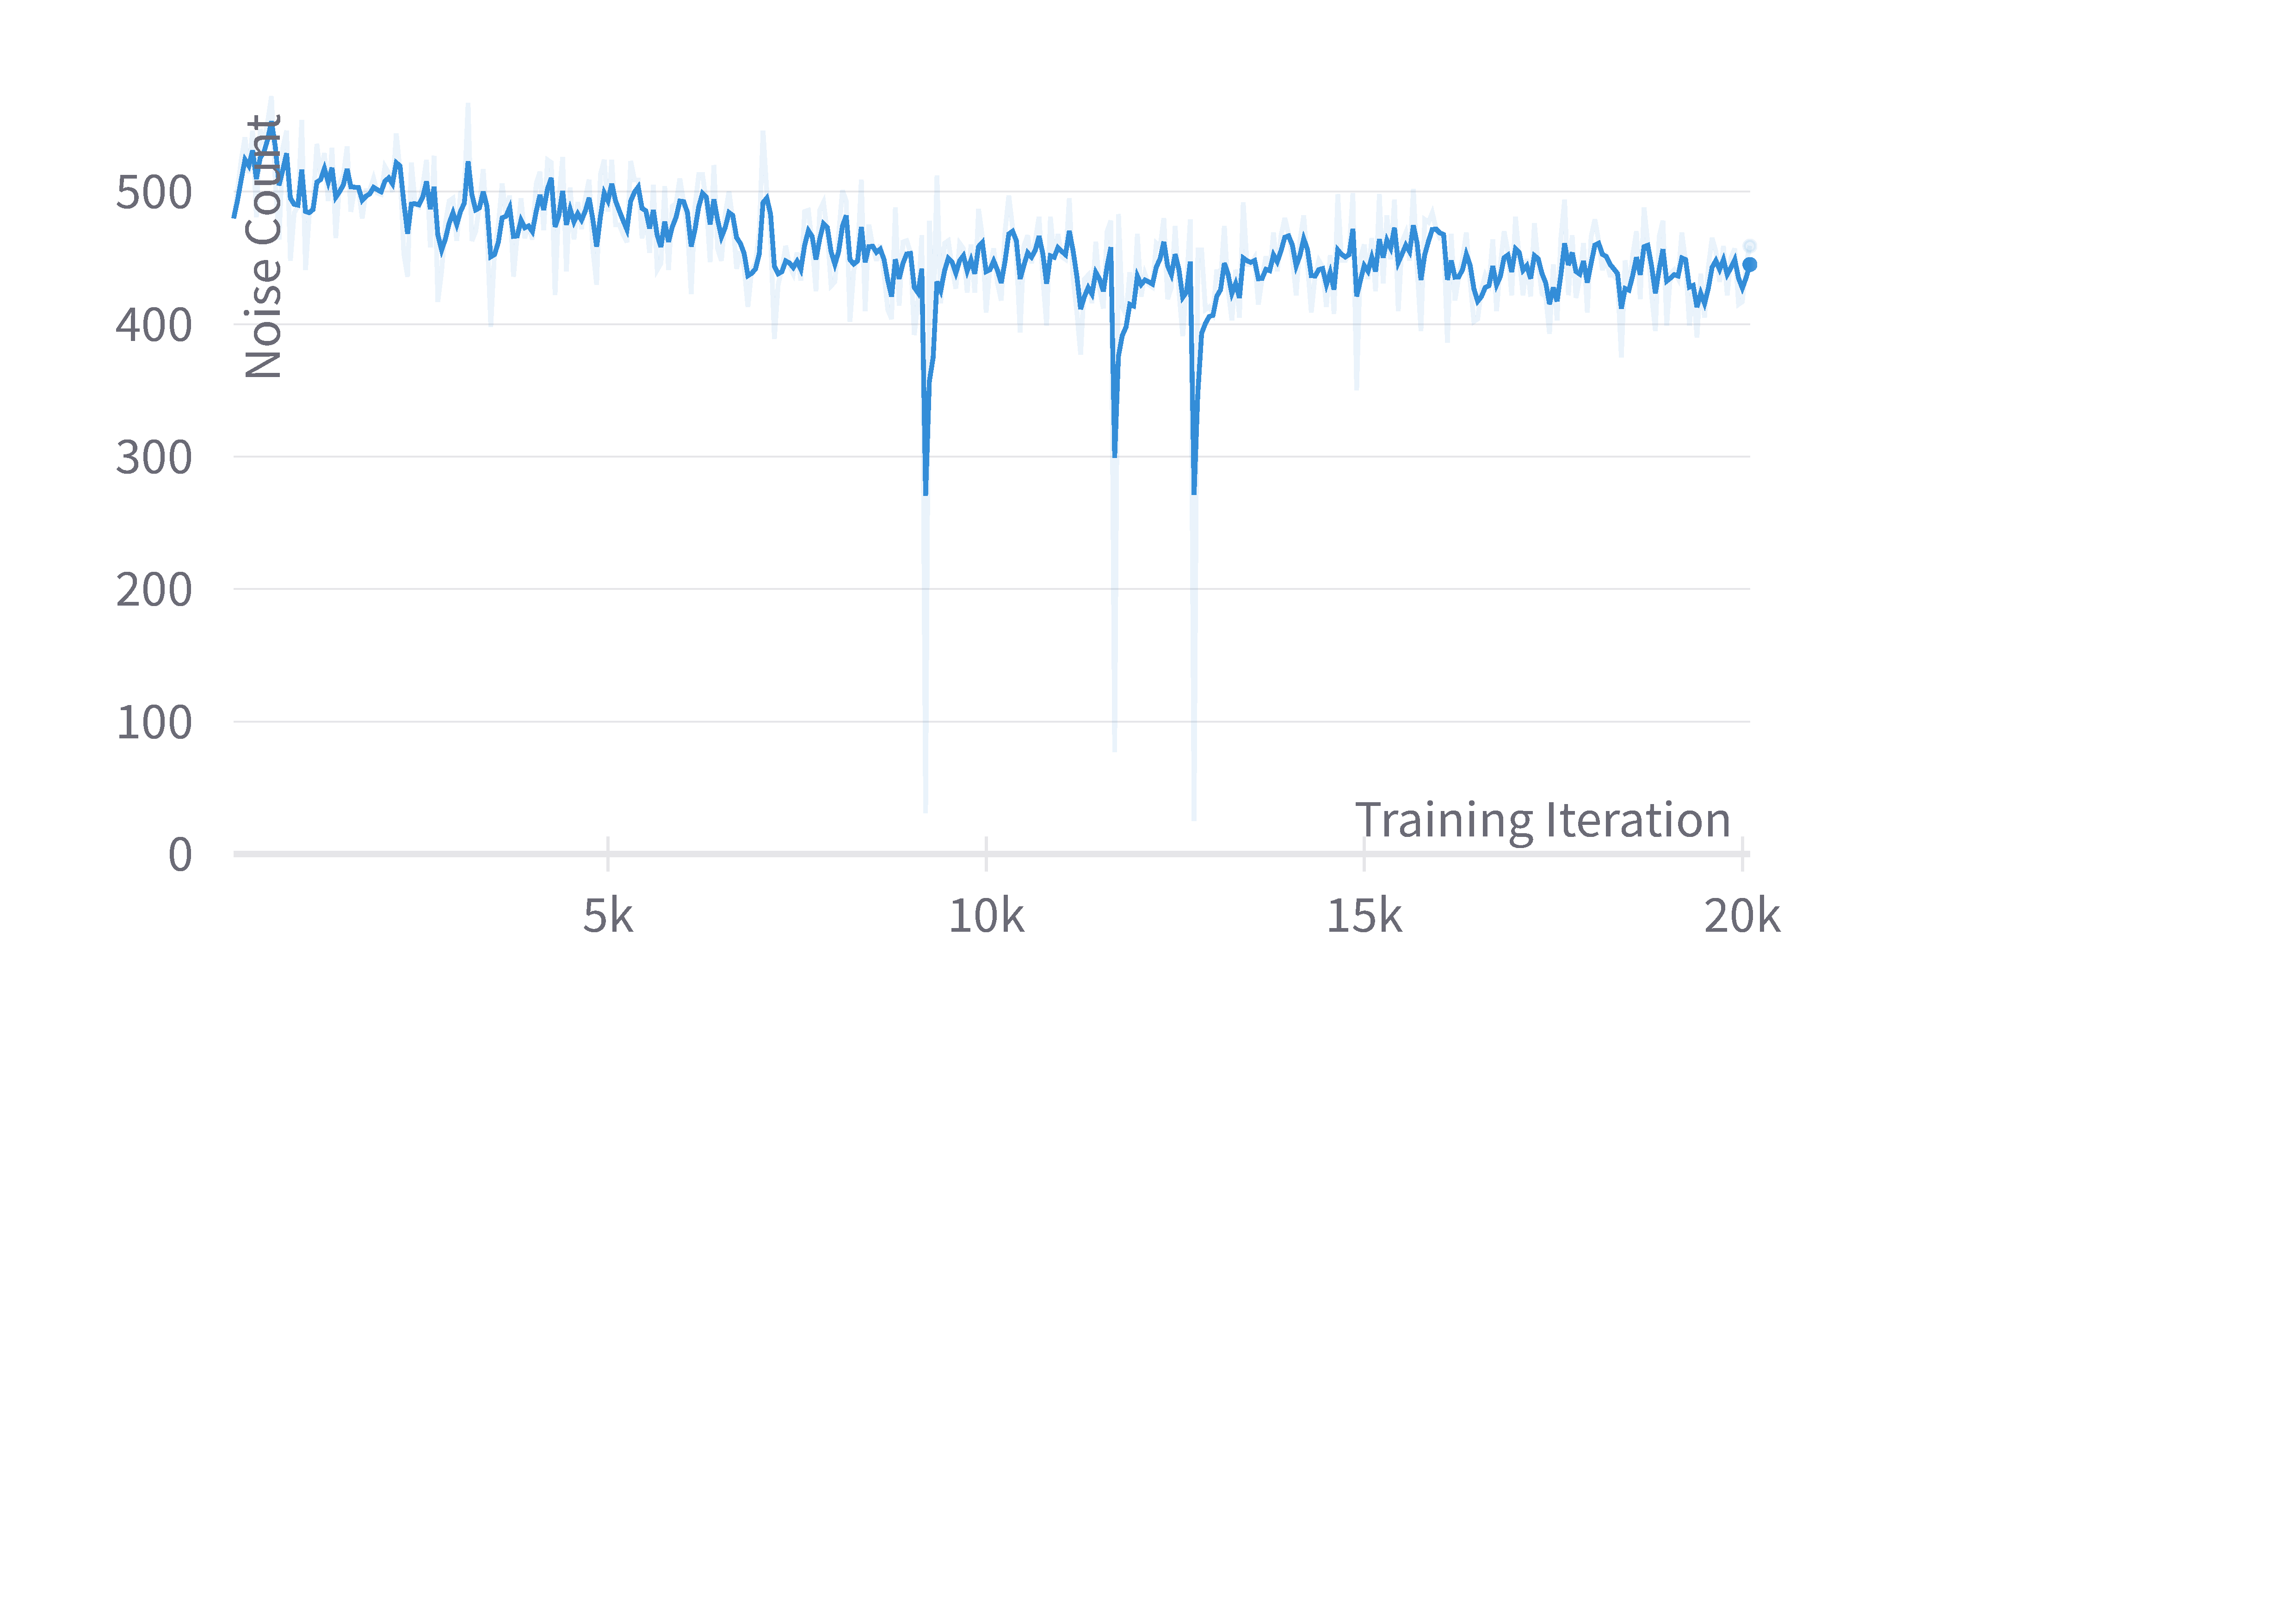
\includegraphics[scale=0.15]{chapters/assets/c3lr_extra/noise_counts.pdf}
    \caption{This graph shows the amount of points clustered as noise by \texttt{HDBSCAN}. We can see that roughly $400$ points are always classified as noise, even after $20,000$ training iterations.}
    \label{fig:hdbscan-noise-count}
\end{figure}

\newpage
\subsection{Partial Compatibility with Gradient Based Learning}\label{ssec:c3lr-grad-based}

A major drawback of \ccclr{} is that the re-ranking and clustering steps are not compatible with gradient based learning. This means that any operations performed by these steps are not recorded in the computational graph tracked by PyTorch \parencite{pytorch2019}. A computational graph keeps track of all mathematical operations performed on a variable; during backpropagation this computational graph is used to calculate the gradients.
Due to this, information that is valuable to the model is lost between lines $8$ and $9$. The loss $\mathcal{L}_1$ is partially able to address this issue, however, it is far from ideal.

\begin{figure}[th]
     \centering
     \begin{subfigure}[b]{0.45\textwidth}
         \centering
         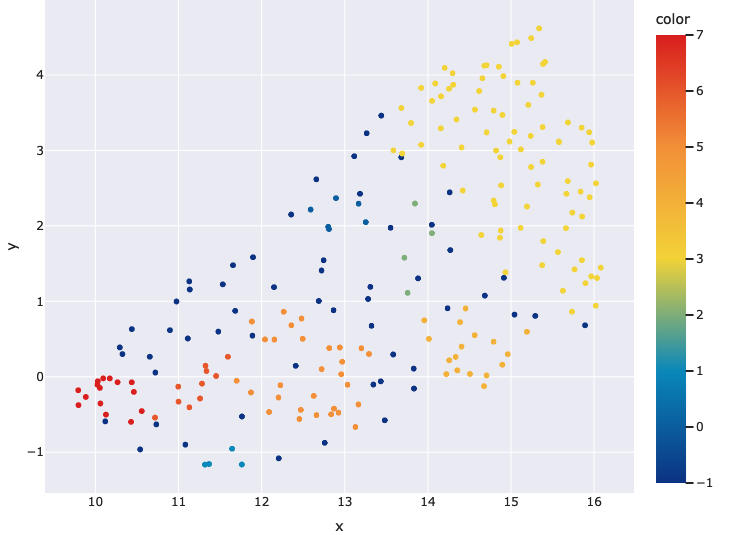
\includegraphics[width=\textwidth]{chapters/assets/c3lr_extra/c1.png}
     \end{subfigure}
     \hspace{1cm}
     \begin{subfigure}[b]{0.45\textwidth}
         \centering
         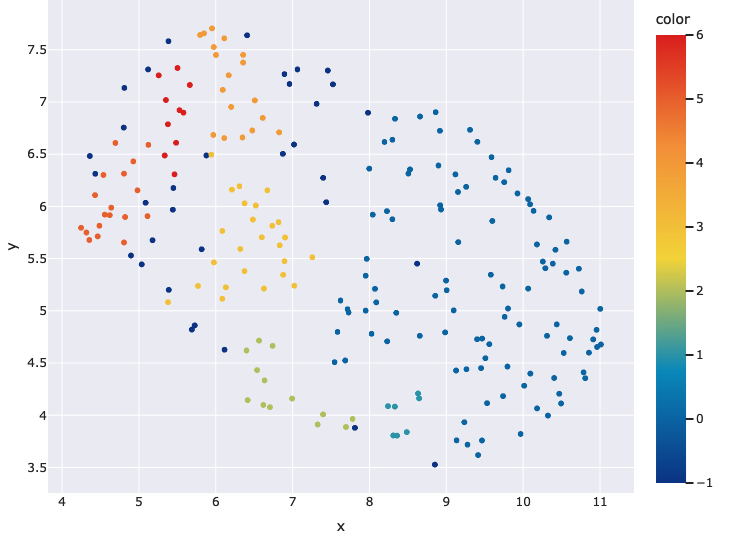
\includegraphics[width=\textwidth]{chapters/assets/c3lr_extra/c2.png}
     \end{subfigure}
     \label{fig:c3lr-hdbscan-results}
     \caption{Two UMAP plots showing the clusters generated by \texttt{HDBSCAN} \parencite{McInnes2017Hdbscan:Clustering}. Notice the massive \textcolor{yellow}{yellow} (left) and \textcolor{blue}{blue} (right) clusters, it is unlikely all elements in them are truly similar. Unfortunately, due to the variable number of clusters generated by \texttt{HDBSCAN}, the legend is shown as a continuous colour scale to avoid repetition of colours. Cluster \textquote{$-1$} contains noisy points.}
\end{figure}